\chapter{Potential Formulation and Radiation}
\section{Scalar and vector potentaial}
Maxwell's equations are
\begin{enumerate}[label=(\roman*)]
	\item $\boldsymbol{\nabla} \cdot \mathbf{E}=\frac{1}{\epsilon_{0}} \rho$
	\item $\boldsymbol{\nabla} \times \mathbf{E}=-\frac{\partial \mathbf{B}}{\partial t}$
	\item $\boldsymbol{\nabla} \cdot \mathbf{B}=0$
	\item $\boldsymbol{\nabla} \times \mathbf{B}=\mu_{0} \mathbf{J}+\mu_{0} \epsilon_{0} \frac{\partial \mathbf{E}}{\partial t}$
\end{enumerate}
If $\rho(r,t)$ and $J(r,t)$ are bnown electric and magnetic field can be find out using Gauss's law and Bio-savart law.It is difficult to find E ans B if they are time dependant.To solve this problem first we are going to represents the fields in terms of potentials electric potential V and magnetic potential B.\\
In the static case $\nabla \times \mathbf{E}=0$ So electric field cane written as a negative gradient of some scalar quandity called electric potential V\\
$$E=-\nabla V$$(not possible in elctrodynamics)\\
But $\nabla \cdot B=0$ always.Which gives \\
$$B=\nabla\times A$$
 Where A is the magnetic vector potential.Putting this value in 
$$\boldsymbol{\nabla} \times \mathbf{E}=-\frac{\partial \mathbf{B}}{\partial t}$$
We will get \\
$$\nabla \times \mathbf{E}=\frac{-\partial }{\partial t}(\nabla \times A)$$
$$\nabla \times \left( \mathbf{E}+\frac{\partial A}{\partial t}\right) =0$$
Again the curl of something become zero. so it can be written as negative gradient of potential
$$\mathbf{E}+\frac{\partial A}{\partial t}=-\nabla V$$
$$\mathbf{E}=-\nabla V-\frac{\partial A}{\partial t}$$
\begin{center}
	\framebox{
		\parbox[t][3cm]{3cm}{
			
			\addvspace{0.2cm} \centering
			
			\begin{align*}
			\begin{array}{lll}
			$$\mathbf{B}=\nabla\times A$$\\
			$$\mathbf{E}=-\nabla V-\frac{\partial A}{\partial t}$$
			\end{array}
			\end{align*}} }
\end{center}
If A and V are known we can find electric and magnetic field with these two equations.

Putting this equation $$\mathbf{E}=-\nabla V-\frac{\partial A}{\partial t}$$  in Gauss's law
we will get,\\
$$\nabla ^2V+\frac{\partial }{\partial t}(\nabla \cdot A)=\frac{-\rho}{\epsilon_{0}}$$
Putting $\mathbf{B}=\nabla\times A$  equation in Ampere/Maxwell's law and rearranging we will get,\\
$$\left( \nabla^2A-\mu_{0}\epsilon_{0}\frac{\partial^2 A}{\partial t^2}\right) -\nabla\left( \nabla \cdot A+\mu_{0}\epsilon_{0}\frac{\partial V}{\partial t}\right) =-\mu_{0} J$$ 

These two equations contain all information in the Maxwell's equations.\\
However we have succeeded in reducing six problems to find E and B ,down to four(V one component,A three component.),these equations are lengthy and difficult to find solution we have to abandon this potential formulation altogether.\\
\paragraph{Gauge transformation}
To avoid this problem we are transforming the potential equations by adding one extra term to A and V.This is called gauge tranformation.Consider the transformation occuring in the same fields E and B.Then\\
$$A^{\prime}=A+\alpha$$ and
$$V^{\prime}=V+\beta$$
Taking curl on each side of $A^{\prime}=A+\alpha$
we will get 
$$\nabla \times A^{\prime}=\nabla \times A+\nabla \times \alpha$$
Since B's are same we can written as($\nabla \times B=0,A^{\prime}=A$) \\
$$\nabla \times \alpha =0$$
Again curl of $\alpha$ is zero.then\\
$$\alpha=\nabla \lambda$$\\
The two potentials also gives the same E.so,\\
$$\nabla \beta +\frac{\partial \alpha }{\partial t}=0$$
$$\nabla\left( \beta+\frac{\partial \lambda}{\partial t}\right) =0$$
$$\beta= -\frac{\partial \lambda}{\partial t}$$
Now transformations become,\\

\begin{center}
	\framebox{
		\parbox[t][3cm]{3cm}{
			
			\addvspace{0.2cm} \centering
			
			\begin{align*}
			\begin{array}{lll}
			 $$A^{\prime}=A+\nabla \lambda$$\\
			 $$V^{\prime}=V-\frac{\partial \lambda}{\partial t}$$
			\end{array}
			\end{align*}} }
\end{center}
\subsection{Coulomb Gauge and Lorentz gauge}
\paragraph{Coluomb gauge}
$$\nabla \cdot A=0$$ is called Coulomb gauge.\\
\paragraph{importance}
$$\nabla \cdot A=0$$ Then the equation 
$$\nabla ^2V+\frac{\partial }{\partial t}(\nabla \cdot A)=\frac{-\rho}{\epsilon_{0}}$$ become,\\
$$\nabla^2 V=\frac{-\rho}{\epsilon_{0}}$$
This is poisson's equation.From this equation V can be findout by using the formula\\
$$V(r,t)=\frac{1}{4 \pi \epsilon_0}\int \frac{\rho(r^{\prime},t)}{r}d\tau^{\prime}$$
V is easy to get but to find E we need  A also($E=-\nabla V-\frac{\partial A}{\partial t}$) which is difficult.
\paragraph{Advantage of the coulomb gauge is that the scalar potential is simply to calculate .The disadvatage is that  A is particularly difficult to calculate. }
After applying coulomb gauge to the equation 
$$\left( \nabla^2A-\mu_{0}\epsilon_{0}\frac{\partial^2 A}{\partial t^2}\right) -\nabla\left( \nabla \cdot A+\mu_{0}\epsilon_{0}\frac{\partial V}{\partial t}\right) =-\mu_{0} J$$ 
we get\\
$$\left( \nabla^2A-\mu_{0}\epsilon_{0}\frac{\partial^2 A}{\partial t^2}\right)=-\mu_{0}J+\mu_{0} \epsilon_{0}\nabla \left( \frac{\partial V}{\partial t}\right) $$
\paragraph{Lorentz gauge}
$$\nabla \cdot A =-\mu_{0} \epsilon_{0} \frac{\partial}{\partial t}V$$

 is called the lorentz gauge.\\
 This designes to eliminate the middle term of the equation
$$\left( \nabla^2A-\mu_{0}\epsilon_{0}\frac{\partial^2 A}{\partial t^2}\right) -\nabla\left( \nabla \cdot A+\mu_{0}\epsilon_{0}\frac{\partial V}{\partial t}\right) =-\mu_{0} J$$
With lorentz gauge this equation become
$$\nabla^2A-\mu_{0}\epsilon_{0}\frac{\partial^2 A}{\partial t^2}=-\mu_{0} J$$
With lorentz gauge this equation 
$\nabla ^2V+\frac{\partial }{\partial t}(\nabla \cdot A)=\frac{-\rho}{\epsilon_{0}}$
becomes
$$\nabla^2A-\mu_{0}\epsilon_{0}\frac{\partial^2 A}{\partial t^2}=\frac{-\rho}{\epsilon_{0}}$$
The virtue of the lorentz gauge is that it treats V and A on the same differential operator
$$\nabla^2-\mu_{0} \epsilon_{0}\frac{\partial ^2}{\partial t^2}\equiv \square^2  $$
 is called d'Alembertian\\
Then both equation become\\
$$\square^2V=\frac{-\rho}{\epsilon_{0}}$$
$$\square^2A=-\mu_{0} J$$
\section{Retarded Potentials}
$$\square^{2} V=-\frac{1}{\epsilon_{0}} \rho, \quad \square^{2} \mathbf{A}=-\mu_{0} \mathbf{J}$$
In static case these equation reduces to poisson's equations
$$\nabla^{2} V=-\frac{1}{\epsilon_{0}} \rho, \quad \nabla^{2} \mathbf{A}=-\mu_{0} \mathbf{J}$$
with solutions
$$V(\mathbf{r})=\frac{1}{4 \pi \epsilon_{0}} \int \frac{\rho\left(\mathbf{r}^{\prime}\right)}{r} d \tau^{\prime}, \quad \mathbf{A}(\mathbf{r})=\frac{\mu_{0}}{4 \pi} \int \frac{\mathbf{J}\left(\mathbf{r}^{\prime}\right)}{r} d \tau^{\prime}$$
$r \rightarrow$ distance from source point $\vec{r}$ to the field point $r$.\\
Imagine a electromagnetic news travels at the speed of light. In non-static case therefore, it's not the status of source right now that matters but rather its condition at some earlier time $t_r$ (retarded time) when the message left.\\
Since the message must travel a distance $r$ the delay is $r/c$
$$t_{r}=t-r / c$$
$\therefore$ Potentials become
$$V(\mathbf{r})=\frac{1}{4 \pi \epsilon_{0}} \int \frac{\rho\left(\mathbf{r}^{\prime}\right)}{r} d \tau^{\prime}, \quad \mathbf{A}(\mathbf{r})=\frac{\mu_{0}}{4 \pi} \int \frac{\mathbf{J}\left(\mathbf{r}^{\prime}\right)}{r} d \tau^{\prime}$$
$P(r^\prime,t_r)$: charge density prevailed at point $r^\prime$ at the retarded time $t_r$. Because the integrants are evaluated at the retarded time these are called retarded potentials.\\
The more distant parts of the charge distribution have earlier retarded times than nearby ones.\\
In calculating the Laplacian of $V(r,t)$\\
The integrand depends on $\vec{r}$ in two places explicitly, in the denomenator $(r=|r-r^\prime|)$ and implicitly through $t_r-t-r/c$ in neumerator 
\begin{align*}
\nabla V&=\frac{1}{4 \pi \epsilon_{0}} \int\left[(\nabla \rho) \frac{1}{r}+\rho \nabla\left(\frac{1}{2}\right)\right] d \tau^{\prime}\\
\nabla \rho&=\dot{\rho} \nabla t_{r}=-\frac{1}{c} \dot{\rho} \nabla r\\
\nabla r&=\hat{r} \text{ and } \nabla \left( \frac{1}{r}\right) =\frac{-\hat{r}}{r^2}\\
\nabla V&=\frac{1}{4 \pi \epsilon_{0}} \int\left[-\frac{\rho}{c} \frac{\hat{r}}{r}-\rho \frac{\hat{\varepsilon}}{r^{2}}\right] d \tau^{\prime}
\intertext{Taking the divergence}
\nabla^{2} V&=\frac{1}{4 \pi \epsilon_{0}} \int\left\{-\frac{1}{c}\left[\frac{\hat{\imath}}{r} \cdot(\nabla \dot{\rho})+\dot{\rho} \nabla \cdot\left(\frac{\hat{r}}{r}\right)\right]\right.
-\left.-\left[\frac{\hat{z}}{r^{2}} \cdot(\nabla \rho)+\rho \nabla \cdot\left(\frac{\hat{\varepsilon}}{r^{2}}\right)\right]\right\} d \tau^{\prime} .\\
\nabla \dot{\rho}&=-\frac{1}{c} \ddot{\rho} \nabla r=-\frac{1}{c} \ddot{\rho} \hat{r},\quad 
\nabla \cdot\left(\frac{\hat{r}}{r}\right)=\frac{1}{r^{2}} 
\intertext{whereas}
&\nabla \cdot\left(\frac{\hat{r}}{r^{2}}\right)=4 \pi \delta^{3}(r)
\intertext{So}
\nabla^{2} V&=\frac{1}{4 \pi \epsilon_{0}} \int\left[\frac{1}{c^{2}} \frac{\ddot{\rho}}{r}-4 \pi \rho \delta^{3}(r)\right] d \tau^{\prime}=\frac{1}{c^{2}} \frac{\partial^{2} V}{\partial t^{2}}-\frac{1}{\epsilon_{0}} \rho(\mathbf{r}, t)\\
\nabla^{2} V&=\frac{1}{c^{2}} \frac{\partial^{2} V}{\partial t^{2}}-\frac{1}{\epsilon_{0}} \rho(\mathbf{r}, t)
\intertext{retarded potential satisfies the inhomogeneous wave equation}
\end{align*}
\section{Jefimentro's Equations}
\begin{align*}
V(r, t)&=\frac{1}{4 \pi \varepsilon_{0}} \int \frac{f\left(r^{\prime}, t_{1}\right)}{r} d z^{\prime},\quad A(r, t)=\frac{\mu_{0}}{4 \pi} \int \frac{J\left(r^{\prime}, t_{r}\right)}{r} d r !
\intertext{It is in principle, a straight forward matter to determine the fields}
E&=-\nabla V-\frac{\partial A}{\partial t}, B=\nabla \times A \\\\
E(r, t)&=\frac{1}{4 \pi \varepsilon_{0}} \int\left[\frac{\rho\left(r^{\prime}, t_{1}\right)}{x^{2}} \hat{x}+\right.\left.\frac{\dot{p}\left(r^{\prime}, t_{1}\right)}{c r} \hat{x}-\frac{\ddot{j}\left(r^{\prime}, t_{1}\right)}{c^{2} r}\right] d \tau^{\prime}
\intertext{This is the time dependent generalization of couloumb's law. In static case the second term and third term drops out and the first term losed its dependence on $t_r$}
B(r, t)&=\frac{\mu_{0}}{4 \pi}\int\left[\frac{J\left(r^{\prime}, f_{r}\right)}{\lambda^{2}}+\frac{J\left(r^{\prime}, t_{r}\right)}{c \lambda}\right]x r^2d z
\intertext{This is the time-denpendent generalzation of the Biot-savart law, to which it reduces in the static case.}
\end{align*}
\section{Poynting Theorem}
If there exist a continuous distribution of charge and current, the total rate of doing work by the fields in a finite volume $v$ is
$$\frac{d w}{d t}=\int_{v} \vec{\j} \cdot \vec{E} d^{3} x$$
This power represent a convertion of electromagnetic energy to mechanical or thermal energy. It must be balanced by corresponding rate  of decrease of energy in the electromagnetic field within the volume $V$. We can use maxwell equations to express the above equation in other terms.
\begin{align*}
\int_{V} J \cdot E d ^3 x&=\int_{V}\left[E \cdot(\nabla x H)-E \cdot \frac{\partial D}{\partial F}\right] d{ }^{3} x\\
\text{using the vector identity}&\\
\nabla \cdot(E \times H)&=H \cdot(\nabla \times \mathbf{E})-E \cdot(\nabla \times H)\\
\because \quad \int_{V} \vec{J} \cdot \vec{E} d^{3} x&=-\int_{V} \bar{V} \cdot(E \times M)+E \cdot \frac{\partial D}{\partial t}+H \cdot \frac{\partial B}{\partial t} \\
\int_{V} \vec{J} \cdot \vec{E} d^{3} x&=-\int_{V}\left[\nabla \cdot(E \times H)+E \cdot \frac{\partial D}{\partial t}+H \cdot \frac{\partial B}{\partial t}\right] d^{3} x
\end{align*}
\textbf{Assumptions}\\
\begin{enumerate}
	\item The mactoscopic medium is lenear in its electric and magnetic properties, with negligible dispersion or losses.
	\item The sum of work necessary to assemble  a static charge distribution and work required to get currents going represent the total deelectromagnetic energy density.
\end{enumerate}
\begin{align*}
u&=\frac{1}{2}(E \cdot D+B \cdot H)\\
-\int_{v} \vec{J} \cdot t^{2} d^{3} x&=\int_{v}\left[\frac{\partial u}{\partial t}+\nabla \cdot(E \times H)\right] d^{3} x
\intertext{since the volume $V$ is arbitrary, this can be cast into the form of a differential contunuity equation or conservation law,}
\frac{\partial u}{\partial t}+\nabla \cdot s&=-j \cdot E\\
\text{The vector $S$ representing }&\text{energy flow is called the poynting vector}\\
S&=E \times H\\
\text{It has diamensions of }&\frac{\text{energy}}{\text{area}\times\text{time}}
\end{align*}
\subsection{Poynting Theorem for Microscopic Fields}
Matter is ultimately composed of charged particles, we can think of this rate of conversion of electromagnetic energy to machanical energy as the rate of increase of energy of charged particles per unit volume\\
We can interpret pointing's theorem for the microscopic fields (E.B) as a statement of conservation of energy of the combined system of particles and fields.\\
Let $E_{mech}$ be the total energy of the particles within the volume $V$ assume no particles move out of the volume.
$$\frac{d E_{\text {mech }}}{d t}=\int_{v} \vec{J} \cdot \vec{E} d^{3} x$$
Poynting theorem express the conservation of energy for the combined system as
$$\frac{d E}{d t}=\frac{d}{d t}\left(E_{\text {mech }}+E_{\text {field }}\right)=-\oint_{s} \vec{n} \cdot \vec{s} d a$$
when the total field energy within $V$ is
$$E_{\text {field } }=\int_{V} u d^{3} x=\frac{\varepsilon_{0}}{2} \int_{V}\left(E^{2}+c^{2} B^{2}\right) d^{3} x$$
\section{Radiation From Moving Charges}
An accelerating or de-accelerating charge producess electro magnetic radiation.
\begin{align*}
\intertext{Produces $EM$ radiation in all direction. There is a $\vec{E} and \vec{B}$ assosiated with it }
\vec{S}&=\frac{1}{\mu_{0}}(\vec{E} \times \vec{B})\\
\text{If $\vec{E}$ and $\vec{B}$ }&\text{are function of time then $\langle\vec{S}\rangle_{t}$ is average of $\vec{S}$}
\end{align*}
\begin{itemize}
	\item Total power radiated through it's surface:
	$$P(x)=\oint_{S}\langle\vec{S}\rangle \cdot d \vec{a}$$
	\item Total power radiated through space:
	$$P=\lim _{r \rightarrow \infty} P(r)$$
	For $\infty$ radius-we get total power radiated.\\
\end{itemize}
\textbf{When particle accelerating in $\hat{z}$ direction}\\
A charge $q$ with mass $m$ that is accelerating with acceleration $a$ along $z$ direction at point $P$ what will be $E$ and $B$.\\
What will be dependense of $E$ and $B$ at $P$
\begin{align*}
|\vec{E}| \propto &\frac{q a \sin \theta}{r}\\
|\vec{B}| \propto &\frac{q \operatorname{asin} \theta}{r}\\
I=|\vec{S}| \propto& \frac{q^{2} a^{2} \sin ^{2} \theta}{r^{2}}\text{dependence of intensity}\\
\text{If average }&\text{pointing vector is given}\\
\langle\vec{S}\rangle&=\frac{\mu_{0} q^{2} a^{2}}{16 \pi^{2} c}\left(\frac{\sin ^{2} \theta}{r^{2}}\right) \hat{r}
\end{align*}
\begin{itemize}
	\item Along $z$-direction intensity is minimum $\rightarrow 0$ ie there is no electro magnetic radiation in $z$ direction. 
	\item Maximum radiation will be in $x-y$ plane.
\end{itemize}
\section{Toral Power Radiated}
\begin{align*}
	P&=\oint_{S}\langle\vec{s}\rangle \cdot d \vec{a}\\
	&=\int_{\theta=0}^{\pi} \int_{\phi=0}^{2 \pi} \frac{\mu_{0} q^{2} a^{2}}{16 \pi^{2} c}\left(\frac{\sin ^{2} \theta}{x^{2}}\right) \hat{r} \cdot r^{2} \sin \theta d \theta d \phi \hat{r}\\
	&=\frac{\mu 0 q^{2} a^{2}}{16 \pi^{2} c} \times 2 \pi \int_{0}^{\pi} \sin ^{3} \theta d \theta\\
	&=\frac{\mu_{0} q^{2} a^{2}}{4 N_{2} \pi C} \times 2 \times \frac{4}{3}\\
	p&=\frac{\mu_{0} q^{2} a^{2}}{6 \pi c}\\
	\text{Here $P$}&\text{ is independent of $r$ }
	\intertext{$\therefore $ total power radiated through surface is the total power radiated in space. }
\end{align*}
\subsection{Direction of $\vec{E}$}
\begin{enumerate}
	\item $\vec{E}$ is $\perp^{r}$ to $\vec{r}$
	\item $\vec{a}, \vec{r}$ and $\vec{E}$ lies in oneplanne
\end{enumerate}
If we know direction of $\vec{E} $ we  can find direction of $\vec{B}$ as $\vec{E}\times\vec{B}$ is in the direction of energy flow
\begin{exercise}
	A non relativistic particle of mass $m$ and charge moving with velocity $\vec{V}$ and acceleration $\vec{a}$ emits radiation of intensity $I$. Another particle of mass $\frac{m}{2}$ charge $2E$ velocity $\frac{V}{2}$ emits radiation of intensity $16 \ I$. Find the acceleration of second particle 
\end{exercise}
\begin{answer}$\left. \right. $\\
\begin{tabular}{p{2cm}p{1cm}p{0.5cm}p{0.5cm}p{0.5cm}p{0.7cm}}
	Particle 1&m&e&$\vec{v}$&a&I\\\\
	Particle 2&$\frac{m}{2}$&2e&$\frac{v}{2}$& &10 I\\
\end{tabular}
\begin{align*}
I_{1} \alpha &= \frac{q_{1}^{2} a _1\sin ^{2} \theta}{r^{2}}\\
I_{2} \alpha &\frac{a_{2}^{2} a_{2}^{2} \sin ^{2} \theta}{r^{2}}=16 I_{1}\\
\frac{I_{2}}{I_{1}}&=\frac{q_{2}^{2} a_{2}^{2}}{q_{1} ^2 a_{1}^{2}}=\frac{(2 e)^{2} a_{2}^{2}}{(e)^{2} a_{1}^{2}}=16\\
\frac{4 a_{2}^{2}}{a_{1}^{2}}&=16\\
a_{2}^{2}&=4 a_{1}{ }^{2}\\
a_{2}&=2 a_{1}\\
a_{2}&=2 a
\end{align*}
\end{answer}
\begin{exercise}
	An electron de-accelerated at a constant rate starting from an initial velocity $u(u<<c)$ to $\frac{u}{2}$ during which it travel a distance $d$. Find the total energy radiated in time $t$.
\end{exercise}
\begin{answer}
	\begin{align*}
	p&=\frac{\mu_{0}q^2 a^2}{6\pi C}\text{total power radiated}\\
	a&=\frac{\frac{u}{2}-u}{t}=\frac{-u}{2t}\\
	a^{2}&= \frac{u^{2}}{4 t^{2}}\\
	p&=\frac{\mu_{0}e^2\frac{u^2}{4t^2}}{6\pi C}\\
	\text{Total energy radiated }&p\times t\\
	E&=\frac{\mu_{0}e^2a^2}{24 \pi ct^2}\times t=\frac{\mu_{0}e^2u^2}{24}
	\end{align*}
\end{answer}























\newpage
\begin{abox}
	Practise Set-1
\end{abox}
\begin{enumerate}
	\item  A For constant uniform electric and magnetic field $\vec{E}=\vec{E}_{0}$ and $\vec{B}=\vec{B}_{0}$, it is possible to choose a gauge such that the scalar potential $\phi$ and vector potential $\vec{A}$ are given by
	{\exyear{NET/JRF(JUNE-2011)}}
	\begin{tasks}(1)
		\task[\textbf{A.}] $\phi=0$ and $\vec{A}=\frac{1}{2}\left(\vec{B}_{0} \times \vec{r}\right)$
		\task[\textbf{B.}] $\phi=-\vec{E}_{0} \cdot \vec{r}$ and $\vec{A}=\frac{1}{2}\left(\vec{B}_{0} \times \vec{r}\right)$
		\task[\textbf{C.}]  $\phi=-\vec{E}_{0} \cdot \vec{r}$ and $\vec{A}=0$
		\task[\textbf{D.}] $\phi=0$ and $\vec{A}=-\vec{E}_{0} t$
	\end{tasks}
	
	\item	D A constant electric current $I$ in an infinitely long straight wire is suddenly switched on at $t=0$. The vector potential at a perpendicular distance $r$ from the wire is given by $\vec{A}=\frac{\hat{k} \mu_{0} I}{2 \pi} \ln \left[\frac{1}{r}\left(c t+\sqrt{c^{2} t^{2}-r^{2}}\right)\right]$. The electric field at a distance $r(<c t)$ is
	{\exyear{NET/JRF(DEC-2011)}}
	\begin{tasks}(2)
		\task[\textbf{A.}] 0
		\task[\textbf{B.}] $\frac{\mu_{0} I}{2 \pi t} \frac{1}{\sqrt{2}}(\hat{i}-\hat{j})$
		\task[\textbf{C.}] $\frac{c \mu_{0} I}{2 \pi \sqrt{c^{2} t^{2}-r^{2}}} \frac{1}{\sqrt{2}}(\hat{i}+\hat{j})$
		\task[\textbf{D.}] $-\frac{c \mu_{0} I}{2 \pi \sqrt{c^{2} t^{2}-r^{2}}} \hat{k}$
	\end{tasks}
	\item D Consider an infinite conducting sheet in the $x y$-plane with a time dependent current density $K t \hat{i}$, where $K$ is a constant. The vector potential at $(x, y, z)$ is given by $\vec{A}=\frac{\mu_{0} K}{4 c}(c t-z)^{2} \hat{i}$. The magnetic field $\vec{B}$ is
	{	\exyear{NET/JRF(DEC-2012)}}
	\begin{tasks}(2)
		\task[\textbf{A.}] $\frac{\mu_{0} K t}{2} \hat{j}$
		\task[\textbf{B.}] $-\frac{\mu_{0} K z}{2 c} \hat{j}$
		\task[\textbf{C.}] $-\frac{\mu_{0} K}{2 c}(c t-z) \hat{i}$
		\task[\textbf{D.}] $-\frac{\mu_{0} K}{2 c}(c t-z) \hat{j}$
	\end{tasks}
	\item C A current $I$ is created by a narrow beam of protons moving in vacuum with constant velocity $\vec{u}$. The direction and magnitude, respectively of the Poynting vector $\vec{S}$ outside the beam at a radial distance $r$ (much larger than the width of the beam) from the axis, are
	{	\exyear{NET/JRF(JUNE-2013)}}
	\begin{tasks}(2)
		\task[\textbf{A.}] $\vec{S} \perp \vec{u}$ and $|\vec{S}|=\frac{I^{2}}{4 \pi^{2} \varepsilon_{0}|\vec{u}| r^{2}}$
		\task[\textbf{B.}] $\vec{S} \|(-\vec{u})$ and $|\vec{S}|=\frac{I^{2}}{4 \pi^{2} \varepsilon_{0}|\vec{u}| r^{4}}$
		\task[\textbf{C.}] $\vec{S} \| \vec{u}$ and $|\vec{S}|=\frac{I^{2}}{4 \pi^{2} \varepsilon_{0}|\vec{u}| r^{2}}$
		\task[\textbf{D.}] $\vec{S} \| \vec{u}$ and $|\vec{S}|=\frac{I^{2}}{4 \pi^{2} \varepsilon_{0}|\vec{u}| r^{4}}$
	\end{tasks}
	\item
	C If the electric and magnetic fields are unchanged when the potential $\vec{A}$ changes (in suitable units) according to $\vec{A} \rightarrow \vec{A}+\hat{r}$, where $\vec{r}=r(t) \hat{r}$, then the scalar potential $\Phi$ must simultaneously change to
	{	\exyear{NET/JRF(JUNE-2013)}}
	\begin{tasks}(4)
		\task[\textbf{A.}] $\Phi-r$
		\task[\textbf{B.}] $\Phi+r$
		\task[\textbf{C.}] $\Phi-\partial \mathrm{r} / \partial t$
		\task[\textbf{D.}] $\Phi+\partial \mathrm{r} / \partial t$
	\end{tasks}
	\item
	A Let $(V, \vec{A})$ and $\left(V^{\prime}, \overrightarrow{A^{\prime}}\right)$ denote two sets of scalar and vector potentials, and $\psi$ is a scalar function. Which of the following transformations leave the electric and magnetic fields (and hence Maxwell's equations) unchanged?
	{\exyear{NET/JRF(DEC-2013)}}
	\begin{tasks}(2)
		\task[\textbf{A.}] $\overrightarrow{A^{\prime}}=\vec{A}+\nabla \psi$ and $V^{\prime}=V-\frac{\partial \psi}{\partial t}$
		\task[\textbf{B.}] $\overrightarrow{A^{\prime}}=\vec{A}-\nabla \psi$ and $V^{\prime}=V+2 \frac{\partial \psi}{\partial t}$
		\task[\textbf{C.}] $\overrightarrow{A^{\prime}}=\vec{A}+\nabla \psi$ and $V^{\prime}=V+\frac{\partial \psi}{\partial t}$
		\task[\textbf{D.}] $\overrightarrow{A^{\prime}}=\vec{A}-\nabla \psi$ and $V^{\prime}=V-\frac{\partial \psi}{\partial t}$
	\end{tasks}
	\item
	A A time-dependent current $\vec{I}(t)=K t \hat{z}$ (where $K$ is a constant) is switched on at $t=0$ in an infinite current-carrying wire. The magnetic vector potential at a perpendicular distance $a$ from the wire is given (for time $t>a / c$ ) by
	{	\exyear{NET/JRF(JUNE-2014)}}
	\begin{tasks}(2)
		\task[\textbf{A.}]  $\hat{z} \frac{\mu_{0} K}{4 \pi c} \int_{-\sqrt{c^{2} t^{2}-a^{2}}}^{\sqrt{c^{2} t^{2}-a^{2}}} d z \frac{c t-\sqrt{a^{2}+z^{2}}}{\left(a^{2}+z^{2}\right)^{1 / 2}}$
		\task[\textbf{B.}]  $\hat{z} \frac{\mu_{0} K}{4 \pi} \int_{-c t}^{c t} d z \frac{t}{\left(a^{2}+z^{2}\right)^{1 / 2}}$
		\task[\textbf{C.}] $\hat{z} \frac{\mu_{0} K}{4 \pi c} \int_{-c t}^{c t} d z \frac{c t-\sqrt{a^{2}+z^{2}}}{\left(a^{2}+z^{2}\right)^{1 / 2}}$
		\task[\textbf{D.}] $\hat{z} \frac{\mu_{0} K}{4 \pi} \int_{-\sqrt{c^{2} t^{2}-a^{2}}}^{\sqrt{c^{2} t^{2}-a^{2}}} d z \frac{t}{\left(a^{2}+z^{2}\right)^{1 / 2}}$
	\end{tasks}
	
	
	\item C The vector potential $\vec{A}=k e^{-a t} r \hat{r}$ (where $a$ and $k$ are constants) corresponding to an electromagnetic field is changed to $\overrightarrow{A^{\prime}}=-k e^{-a t} r \hat{r}$. This will be a gauge transformation if the corresponding change $\phi^{\prime}-\phi$ in the scalar potential is
	{\exyear{NET/JRF(JUNE-2017)}}
	\begin{tasks}(4)
		\task[\textbf{A.}] $a k r^{2} e^{-a t}$
		\task[\textbf{B.}] $2 a k r^{2} e^{-a t}$
		\task[\textbf{C.}] $-a k r^{2} e^{-a t}$
		\task[\textbf{D.}] $-2 a k r^{2} e^{-a t}$
	\end{tasks}
	\item A The charge distribution inside a material of conductivity $\sigma$ and permittivity $\in$ at initial time $t=0$ is $\rho(r, 0)=\rho_{0}$, a constant. At subsequent times $\rho(r, t)$ is given by
	{\exyear{NET/JRF(JUNE-2017)}}
	\begin{tasks}(2)
		\task[\textbf{A.}]  $\rho_{0} \exp \left(-\frac{\sigma t}{\epsilon}\right)$
		\task[\textbf{B.}] $\frac{1}{2} \rho_{0}\left[1+\exp \left(\frac{\sigma t}{\in}\right)\right]$
		\task[\textbf{C.}]  $\frac{\rho_{0}}{\left[1-\exp \left(\frac{\sigma t}{\epsilon}\right)\right]}$
		\task[\textbf{D.}] $\rho_{0} \cosh \frac{\sigma t}{\in}$
	\end{tasks}
	\item  B The electric field $\vec{E}$ and the magnetic field $\vec{B}$ corresponding to the scalar and vector potentials, $V(x, y, z, t)=0$ and $\vec{A}(x, y, z, t)=\frac{1}{2} \hat{k} \mu_{0} A_{0}(c t-x)$, where $A_{0}$ is a constant, are 
	{\exyear{NET/JRF(JUNE-2018)}}
	\begin{tasks}(2)
		\task[\textbf{A.}] (a) $\vec{E}=0$ and $\vec{B}=\frac{1}{2} \hat{j} \mu_{0} A_{0}$
		\task[\textbf{B.}] $\vec{E}=-\frac{1}{2} \hat{k} \mu_{0} A_{0} c$ and $\vec{B}=\frac{1}{2} \hat{j} \mu_{0} A_{0}$
		\task[\textbf{C.}]  $\vec{E}=0$ and $\vec{B}=-\frac{1}{2} \hat{i} \mu_{0} A_{0}$
		\task[\textbf{D.}] $\vec{E}=\frac{1}{2} \hat{k} \mu_{0} A_{0} c$ and $\vec{B}=-\frac{1}{2} \hat{i} \mu_{0} A_{0}$
	\end{tasks}
\item D Which of the following transformations $(V, \vec{A}) \rightarrow\left(V^{\prime}, \overrightarrow{A^{\prime}}\right)$ of the electrostatic potential $V$ and the vector potential $\vec{A}$ is a gauge transformation?
{\exyear{ NET/JRF-(JUNE-2015)}}
 \begin{tasks}(2)
	\task[\textbf{a.}]$\left(V^{\prime}=V+a x, \vec{A}^{\prime}=\vec{A}+a t \hat{k}\right)$
	\task[\textbf{b.}]$\left(V^{\prime}=V+a x, \vec{A}^{\prime}=\vec{A}-a t \hat{k}\right)$
	\task[\textbf{c.}]$\left(V^{\prime}=V+a x, \vec{A}^{\prime}=\vec{A}+a t \hat{i}\right)$
	\task[\textbf{d.}] $\left(V^{\prime}=V+a x, \vec{A}^{\prime}=\vec{A}-a t \hat{i}\right)$
\end{tasks}
\item D Consider an infinite conducting sheet in the $x y$-plane with a time dependent current density $K t \hat{i}$, where $K$ is a constant. The vector potential at $(x, y, z)$ is given by $\vec{A}=\frac{\mu_{0} K}{4 c}(c t-z)^{2} \hat{i}$. The magnetic field $\vec{B}$ is
{\exyear{NET/JRF-(DEC-2012)}}
 \begin{tasks}(2)
	\task[\textbf{a.}]$\frac{\mu_{0} K t}{2} \hat{j}$
	\task[\textbf{b.}]$-\frac{\mu_{0} K z}{2 c} \hat{j}$
	\task[\textbf{c.}] $-\frac{\mu_{0} K}{2 c}(c t-z) \hat{i}$
	\task[\textbf{d.}]  $-\frac{\mu_{0} K}{2 c}(c t-z) \hat{j}$
\end{tasks}
\item A For constant uniform electric and magnetic field $\vec{E}=\vec{E}_{0}$ and $\vec{B}=\vec{B}_{0}$, it is possible to choose a gauge such that the scalar potential $\phi$ and vector potential $\vec{A}$ are given by 
{\exyear{NET/JRF-(JUNE-2011)}}
 \begin{tasks}(2)
	\task[\textbf{a.}]$\phi=0$ and $\vec{A}=\frac{1}{2}\left(\vec{B}_{0} \times \vec{r}\right)$
	\task[\textbf{b.}]$\phi=-\vec{E}_{0} \cdot \vec{r}$ and $\vec{A}=\frac{1}{2}\left(\vec{B}_{0} \times \vec{r}\right)$
	\task[\textbf{c.}]$\phi=-\vec{E}_{0} \cdot \vec{r}$ and $\vec{A}=0$
	\task[\textbf{d.}] $\phi=0$ and $\vec{A}=-\vec{E}_{0} t$
\end{tasks}
\item C When a charged particle emits electromagnetic radiation, the electric field $\vec{E}$ and the Poynting vector $\vec{S}=\frac{1}{\mu_{0}} \vec{E} \times \vec{B}$ at a larger distance $r$ from emitter vary as $\frac{1}{r^{n}}$ and $\frac{1}{r^{m}}$ respectively. Which of the following choices for $n$ and $m$ are correct?
{\exyear{ NET/JRF-(DEC-2012)}}
 \begin{tasks}(2)
	\task[\textbf{a.}]$n=1$ and $m=1$
	\task[\textbf{b.}] $n=2$ and $m=2$
	\task[\textbf{c.}]$n=1$ and $m=2$
	\task[\textbf{d.}] $n=2$ and $m=4$
\end{tasks}
\item A A non-relativistic particle of mass $m$ and charge $e$, moving with a velocity $\vec{v}$ and acceleration $\vec{a}$, emits radiation of intensity $I$. What is the intensity of the radiation emitted by a particle of mass $m / 2$, charge $2 e$, velocity $\vec{v} / 2$ and acceleration $2 \vec{a}$ ?
{\exyear{NET/JRF-(DEC-2014)}}
 \begin{tasks}(2)
	\task[\textbf{a.}] $16 I$
	\task[\textbf{b.}]$8 I$
	\task[\textbf{c.}]$4 I$
	\task[\textbf{d.}] $2 I$
\end{tasks}
\item D An electron is decelerated at a constant rate starting from an initial velocity $u$ (where $u<<c$ ) to $u / 2$ during which it travels a distance $s$. The amount of energy lost to radiation is
{\exyear{ NET/JRF-(JUNE-2017)}}
 \begin{tasks}(2)
	\task[\textbf{a.}]$\frac{\mu_{0} e^{2} u^{2}}{3 \pi m c^{2} s}$
	\task[\textbf{b.}]$\frac{\mu_{0} e^{2} u^{2}}{6 \pi m c^{2} s}$
	\task[\textbf{c.}]$\frac{\mu_{0} e^{2} u}{8 \pi m c s}$
	\task[\textbf{d.}] $\frac{\mu_{0} e^{2} u}{16 \pi m c s}$
\end{tasks}
\item B In the region far from a source, the time dependent electric field at a point $(r, \theta, \phi)$ is
$$
\vec{E}(r, \theta, \phi)=\hat{\phi} E_{0} \omega^{2}\left(\frac{\sin \theta}{r}\right) \cos \left[\omega\left(t-\frac{r}{c}\right)\right]
$$
where $\omega$ is angular frequency of the source. The total power radiated (averaged over a cycle) is
{\exyear{ NET/JRF-(JUNE-2018)}}
 \begin{tasks}(2)
	\task[\textbf{a.}]$\frac{2 \pi}{3} \frac{E_{0}^{2} \omega^{4}}{\mu_{0} c}$
	\task[\textbf{b.}]$\frac{4 \pi}{3} \frac{E_{0}^{2} \omega^{4}}{\mu_{0} c}$
	\task[\textbf{c.}] $\frac{4}{3 \pi} \frac{E_{0}^{2} \omega^{4}}{\mu_{0} c}$
	\task[\textbf{d.}] $\frac{2}{3} \frac{E_{0}^{2} \omega^{4}}{\mu_{0} c}$
\end{tasks}
\item B A dipole of moment $\vec{p}$, oscillating at frequency $\omega$, radiates spherical waves. The vector potential at large distance is
$$
\vec{A}(\vec{r})=\frac{\mu_{0}}{4 \pi} i \omega \frac{e^{i k r}}{r} \vec{p}
$$
To order $\left(\frac{1}{r}\right)$ the magnetic field $\vec{B}$ at a point $\vec{r}=r \hat{n}$ is
{\exyear{ NET/JRF-(DEC-2015)}}
 \begin{tasks}(2)
	\task[\textbf{a.}]$-\frac{\mu_{0}}{4 \pi} \frac{\omega^{2}}{C}(\hat{n} \cdot \vec{p}) \hat{n} \frac{e^{i k r}}{r}$
	\task[\textbf{b.}] $-\frac{\mu_{0}}{4 \pi} \frac{\omega^{2}}{C}(\hat{n} \times \vec{p}) \frac{e^{i k r}}{r}$
	\task[\textbf{c.}] $-\frac{\mu_{0}}{4 \pi} \omega^{2} k(\hat{n} \cdot \vec{p}) \vec{p} \frac{e^{i k r}}{r}$
	\task[\textbf{d.}] $-\frac{\pi_{0}}{4 \pi} \frac{\omega^{2}}{C} \vec{p} \frac{e^{i k r}}{r}$
\end{tasks}
\item D An oscillating current $I(t)=I_{0} \exp (-i \omega t)$ flows in the direction of the $y$-axis through a thin metal sheet of area $1.0 \mathrm{~cm}^{2}$ kept in the $x y$-plane. The rate of total energy radiated per unit area from the surfaces of the metal sheet at a distance of $100 \mathrm{~m}$ is
{\exyear{ NET/JRF-(JUNE-2013)}}
 \begin{tasks}(2)
	\task[\textbf{a.}]$I_{0} \omega /\left(12 \pi \varepsilon_{0} c^{3}\right)$
	\task[\textbf{b.}]$I_{0}^{2} \omega^{2} /\left(12 \pi \varepsilon_{0} c^{3}\right)$
	\task[\textbf{c.}]$I_{0}^{2} \omega^{3} /\left(12 \pi \varepsilon_{0} c^{3}\right)$
	\task[\textbf{d.}] $I_{0}^{2} \omega^{4} /\left(12 \pi \varepsilon_{0} c^{3}\right)$
\end{tasks}
\item B An alternating current $I(t)=I_{0} \cos (\omega t)$ flows through a circular wire loop of radius $R$, lying in the $x y$-plane, and centered at the origin. The electric field $\vec{E}(\vec{r}, t)$ and the magnetic field $\vec{B}(\vec{r}, t)$ are measured at a point $\vec{r}$ such that $r \gg \frac{c}{\omega} \gg R$, where $\vec{r}=|\vec{r}|$.
Which one of the following statements is correct?
{\exyear{ NET/JRF-(DEC-2019)}}
 \begin{tasks}(2)
	\task[\textbf{a.}] The time-averaged $|\vec{E}(\vec{r}, t)| \propto \frac{1}{r^{2}}$
	\task[\textbf{b.}]The time-averaged $|\vec{E}(\vec{r}, t)| \propto \omega^{2}$
	\task[\textbf{c.}]The time-averaged $|\vec{B}(\vec{r}, t)|$ as a function of the polar angle $\theta$ has a minimum at $\theta=\frac{\pi}{2}$
	\task[\textbf{d.}] $\vec{B}(\vec{r}, t)$ is along the azimuthal direction
\end{tasks}
\item  C A particle with charge $-q$ moves with a uniform angular velocity $\omega$ in a circular orbit of radius $a$ in the $x y$ - plane, around a fixed charge $+q$, which is at the centre of the orbit at $(0,0,0)$. Let the intensity of radiation at the point $(0,0, R)$ be $I_{1}$ and at $(2 R, 0,0)$ be ' $I_{2}$ The ratio $\frac{I_{2}}{I_{1}}$ for $R \gg a$, is
{\exyear{NET/JRF-(DEC-2016)}}
 \begin{tasks}(2)
	\task[\textbf{a.}]4
	\task[\textbf{b.}]$\frac{1}{4}$
	\task[\textbf{c.}]$\frac{1}{8}$
	\task[\textbf{d.}]8 
\end{tasks}
\item A The phase difference between two small oscillating electric dipoles, separated by a distance $d$, is $\pi$. If the wavelength of the radiation is $\lambda$, the condition for constructive interference between the two dipolar radiations at a point $P$ when $r \gg d$ (symbols are as shown in the figure and $n$ is an integer) is
{\exyear{NET/JRF-(DEC-2019)}}
\begin{figure}[H]
	\centering
	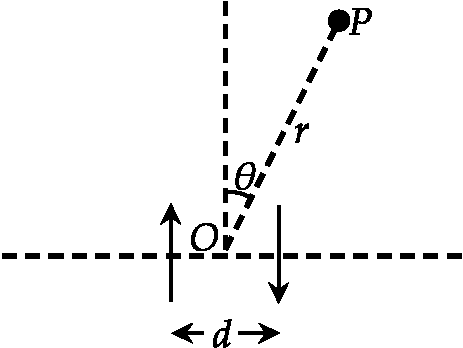
\includegraphics[height=3.2cm,width=5cm]{ED21}
\end{figure}
 \begin{tasks}(2)
	\task[\textbf{a.}]$d \sin \theta=\left(n+\frac{1}{2}\right) \lambda$
	\task[\textbf{b.}]$d \sin \theta=n \lambda$
	\task[\textbf{c.}] $d \cos \theta=n \lambda$
	\task[\textbf{d.}] $d \cos \theta=\left(n+\frac{1}{2}\right) \lambda$
\end{tasks}
\end{enumerate}
 \colorlet{ocre1}{ocre!70!}
\colorlet{ocrel}{ocre!30!}
\setlength\arrayrulewidth{1pt}
\begin{table}[H]
	\centering
	\arrayrulecolor{ocre}
	\begin{tabular}{|p{1.5cm}|p{1.5cm}||p{1.5cm}|p{1.5cm}|}
		\hline
		\multicolumn{4}{|c|}{\textbf{Answer key}}\\\hline\hline
		\rowcolor{ocrel}Q.No.&Answer&Q.No.&Answer\\\hline
		1&\textbf{a} &2&\textbf{d}\\\hline 
		3&\textbf{d} &4&\textbf{c} \\\hline
		5&\textbf{c} &6&\textbf{a} \\\hline
		7&\textbf{a}&8&\textbf{c}\\\hline
		9&\textbf{a}&10&\textbf{b}\\\hline
		11&\textbf{d} &12&\textbf{d}\\\hline
		13&\textbf{a}&14&\textbf{c}\\\hline
		15&\textbf{a}&16&\textbf{d} \\\hline
		17&\textbf{b}&18&\textbf{b}\\\hline
		19&\textbf{d}&20&\textbf{b}\\\hline
		21&\textbf{c} &22&\textbf{a}\\\hline
	\end{tabular}
\end{table}


\newpage
\begin{abox}
	Practise Set-2
\end{abox}
\begin{enumerate}
	\begin{minipage}{\textwidth}
		\item  D The electric and the magnetic field $\vec{E}(z, t)$ and $\vec{B}(z, t)$, respectively corresponding to the scalar potential $\phi(z, t)=0$ and vector potential $\vec{A}(z, t)=\hat{i} t z$ are
		\exyear{GATE 2012}
	\end{minipage}
	\begin{tasks}(2)
		\task[\textbf{A.}] $\vec{E}=\hat{i} z$ and $\vec{B}=-\hat{j} t$
		\task[\textbf{B.}]$\vec{E}=\hat{i} z$ and $\vec{B}=\hat{j t}$
		\task[\textbf{C.}]$\vec{E}=-\hat{i} z$ and $\vec{B}=-\hat{j t}$
		\task[\textbf{D.}]$\vec{E}=-\hat{i} z$ and $\vec{B}=-\hat{j} \mathrm{t}$
	\end{tasks}
	\begin{minipage}{\textwidth}
		\item If the vector potential $\vec{A}=\alpha x \hat{x}+2 y \hat{y}-3 z \hat{z}$, satisfies the Coulomb gauge, the value of the constant $\alpha$ is
		\exyear{GATE 2015}
	\end{minipage}
	\begin{minipage}{\textwidth}
		\item Consider magnetic vector potential $\tilde{A}$ and scalar potential $\Phi$ which define the magnetic field $\vec{B}$ and electric field $\vec{E}$. If one adds $\vec{\nabla} \lambda$ to $\vec{A}$ for a well-defined $\lambda$, then what should be added to $\Phi$ so that $\vec{E}$ remains unchanged up to an arbitrary function of time, $f(t)$ ?
		\exyear{JEST 2017}
	\end{minipage}
	\begin{tasks}(2)
		\task[\textbf{A.}] $\frac{\partial \lambda}{\partial t}$
		\task[\textbf{B.}]$-\frac{\partial \lambda}{\partial t}$
		\task[\textbf{C.}]$\frac{1}{2} \frac{\partial \lambda}{\partial t}$
		\task[\textbf{D.}]$-\frac{1}{2} \frac{\partial \lambda}{\partial t}$
	\end{tasks}
	\item A long straight wire, having radius $a$ and resistance per unit length $r$, carries a current $I$. The magnitude and direction of the Poynting vector on the surface of the wire is
	{\exyear{GATE 2018}}
	\begin{tasks}(1)
		\task[\textbf{A.}] $I^{2} r / 2 \pi a$, perpendicular to axis of the wire and pointing inwards
		\task[\textbf{B.}]$I^{2} r / 2 \pi a$, perpendicular to axis of the wire and pointing outwards
		\task[\textbf{C.}]$I^{2} r / \pi a$, perpendicular to axis of the wire and pointing inwards
		\task[\textbf{D.}]$I^{2} r / \pi a$, perpendicular to axis of the wire and pointing outwards
	\end{tasks}
\item D An electromagnetic field is given by
$$
\vec{E}(\vec{r}, t)=-\frac{1}{4 \pi \in_{0}} \frac{q}{r^{2}} \theta(v t-r) \dot{r}, \quad \vec{B}(\vec{r}, t)=0
$$
where $\theta(x)= \begin{cases}1 & \text { for } x>0 \\ 0 & \text { for } x \leq 0\end{cases}$
The corresponding charge density $\rho$ and current density $\vec{J}$ are given by
{\exyear{ JEST-2020}}
 \begin{tasks}(2)
	\task[\textbf{a.}]$\rho=-q \delta^{3}(\vec{r}) \theta(v t-r)+\frac{q}{4 \pi r^{2}} \theta(v t-r) ; \vec{J}=0$
	\task[\textbf{b.}]$\rho=-q \delta^{3}(\vec{r}) \theta(v t-r) ; \vec{J}=0$
	\task[\textbf{c.}]$\rho=\frac{q}{4 \pi r^{2}} \delta(v t-r) ; \vec{J}=\frac{q v}{4 \pi r^{2}} \delta(v t-r) \hat{r}$
	\task[\textbf{d.}] $\rho=-q \delta^{3}(\vec{r}) \theta(v t-r)+\frac{q}{4 \pi r^{2}} \delta(v t-r) ; \vec{J}=\frac{q v}{4 \pi r^{2}} \delta(v t-r) \hat{r}$
\end{tasks}
\item A Consider magnetic vector potential $\vec{A}$ and scalar potential $\Phi$ which define the magnetic field $\vec{B}$ and electric field $\vec{E}$. If one adds $-\vec{\nabla} \lambda$ to $\vec{A}$ for a well-defined $\lambda$, then what should be added to $\Phi$ so that $\vec{E}$ remains unchanged up to an arbitrary function of time, $f(t)$ ?
{\exyear{ JEST-2017}}
 \begin{tasks}(2)
	\task[\textbf{a.}]$\frac{\partial \lambda}{\partial t}$
	\task[\textbf{b.}]$-\frac{\partial \lambda}{\partial t}$
	\task[\textbf{c.}] $\frac{1}{2} \frac{\partial \lambda}{\partial t}$
	\task[\textbf{d.}]  $-\frac{1}{2} \frac{\partial \lambda}{\partial t}$
\end{tasks}
\item C The electric and magnetic field caused by an accelerated charged particle are found to scale as $E \propto r^{-n}$ and $B \propto r^{-m}$ at large distances. What are the value of $n$ and $m$ ?
{\exyear{ JEST-2013}}
 \begin{tasks}(2)
	\task[\textbf{a.}]$n=1, m=2$
	\task[\textbf{b.}]$n=2, m=1$
	\task[\textbf{c.}]$n=1, m=1$
	\task[\textbf{d.}]$n=2, m=2$
\end{tasks}
\item A An electron is executing simple harmonic motion along the $y$-axis in right handed coordinate system. Which of the following statements is true for emitted radiation?
{\exyear{ JEST-2014}}
 \begin{tasks}(2)
	\task[\textbf{a.}]The radiation will be most intense in $x z$ plane
	\task[\textbf{b.}] The radiation will be most intense in $x y$ plane
	\task[\textbf{c.}]The radiation will violate causality
	\task[\textbf{d.}] The electron's rest mass energy will reduce due to radiation loss
\end{tasks}
\end{enumerate}



\newpage
\begin{abox}
	Practise Set-3
\end{abox}
\begin{enumerate}
	\item The vector potential $\vec{A}=3 k e^{-a t} r \hat{r}$ (where $a$ and $k$ are constants) corresponding to an electromagnetic field is changed to $\vec{A}^{\prime}=-3 k e^{-a t} r \hat{r}$. Under gauge transformation find the corresponding change $\phi^{\prime}-\phi$ in the scalar potential.
	\begin{answer}
		\begin{align*}
		\text { Gauge Transformation } \vec{A}^{\prime}&=\vec{A}+\vec{\nabla} \lambda, \phi^{\prime}=\phi-\frac{\partial \lambda}{\partial t}\\
		\vec{A}-\vec{A}&=-6 k e^{-a t} r \hat{r}=\vec{\nabla} \lambda=\frac{\partial \lambda}{\partial r} \hat{r} \\
		\Rightarrow \lambda&=-3 k e^{-a t} r^{2} \Rightarrow \frac{\partial \lambda}{\partial t}=3 k a e^{-a t} r^{2} \Rightarrow \phi^{\prime}-\phi=-\frac{\partial \lambda}{\partial t}=-3 k a e^{-a t} r^{2}
		\end{align*}
	\end{answer}
	\item If the electric and magnetic fields are unchanged when the potential $\vec{A}$ changes (in suitable units) according to $\vec{A} \rightarrow \vec{A}+2 \hat{r}$, then the scalar potential $\Phi$ must simultaneously change to $\Phi^{\prime}$. Then find $\Phi^{\prime}$.
	\begin{answer}
		\begin{align*}
		\overrightarrow{A^{\prime}}&=\vec{A}+\vec{\nabla} \lambda=\vec{A}+\hat{r} \Rightarrow \partial \lambda / \partial r=2 \Rightarrow \lambda=2 r+C\\
		\Phi^{\prime}&=\Phi-\partial \lambda / \partial t=\Phi-2 \partial r / \partial t
		\end{align*}
	\end{answer}
	\item A dipole is oscillating in z-direction such that the retarded potentials are
	$$
	V(r, \theta, t)=\frac{p_{0} \cos \theta}{4 \pi \varepsilon_{0} r}\left\{-\frac{\omega}{c} \sin \omega\left(t-\frac{r}{c}\right)+\frac{1}{r} \cos \omega\left(t-\frac{r}{c}\right)\right\}
	$$
	and $\vec{A}(r, \theta, t)=-\frac{\mu_{0} p_{0} \omega}{4 \pi r} \sin \left[\omega\left(t-\frac{r}{c}\right)\right] \hat{z}$
	where $r$ and $\theta$ are usual spherical polar coordinate.
	Check that they satisfy the Lorentz gauge condition.
	\begin{answer}
		\begin{align*}
		&\text { Lets check }\text{Lorentz gauge condition } \vec{\nabla} \cdot \vec{A}=-\mu_{0} \varepsilon_{0} \frac{\partial V}{\partial t} \text {. }\\
		&\text { In spherical}\text{ polar coordinate system }\\
		&\vec{A}(r, \theta, t)=-\frac{\mu_{0} p_{0} \omega}{4 \pi r} \sin \left[\omega\left(t-\frac{r}{c}\right)\right](\cos \theta \hat{r}-\sin \theta \hat{\theta})\\
		\vec{\nabla} \cdot \vec{A}&=\frac{1}{r^{2}} \frac{\partial}{\partial r}\left[r^{2} \times-\frac{\mu_{0} p_{0} \omega}{4 \pi r} \sin \omega\left(t-\frac{r}{c}\right) \cos \theta\right]+\frac{1}{r \sin \theta} \frac{\partial}{\partial \theta}\left[\sin \theta \times-\frac{\mu_{0} p_{0} \omega}{4 \pi r} \sin \omega\left(t-\frac{r}{c}\right) \sin \theta\right] \\
		\vec{\nabla} \cdot \vec{A}&=-\frac{\mu_{0} p_{0} \omega}{4 \pi} \frac{1}{r^{2}}\left[\sin \omega\left(t-\frac{r}{c}\right) \cos \theta-\frac{\omega r}{c} \cos \omega\left(t-\frac{r}{c}\right) \cos \theta\right]-\frac{\mu_{0} p_{0} \omega}{4 \pi} \frac{1}{r^{2}}\left[2 \cos \theta \times \sin \omega\left(t-\frac{r}{c}\right)\right] \\
		\vec{\nabla} \cdot \vec{A}&=\frac{\mu_{0} p_{0} \omega}{4 \pi} \frac{1}{r^{2}}\left[\sin \omega\left(t-\frac{r}{c}\right) \cos \theta+\frac{\omega r}{c} \cos \omega\left(t-\frac{r}{c}\right) \cos \theta\right] \\
		&\because V(r, \theta, t)=\frac{p_{0} \cos \theta}{4 \pi \varepsilon_{0} r}\left\{-\frac{\omega}{c} \sin \omega\left(t-\frac{r}{c}\right)+\frac{1}{r} \cos \omega\left(t-\frac{r}{c}\right)\right\}\\
		&\Rightarrow \frac{\partial V}{\partial t}=\frac{p_{0} \cos \theta}{4 \pi \varepsilon_{0} r}\left\{-\frac{\omega^{2}}{c} \cos \omega\left(t-\frac{r}{c}\right)-\frac{\omega}{r} \sin \omega\left(t-\frac{r}{c}\right)\right\} \\
		&\Rightarrow-\mu_{0} \varepsilon_{0} \frac{\partial V}{\partial t}=\frac{\mu_{0} p_{0} \omega}{4 \pi \varepsilon_{0} r^{2}}\left\{\sin \omega\left(t-\frac{r}{c}\right) \cos \theta+\frac{\omega r}{c} \cos \omega\left(t-\frac{r}{c}\right) \cos \theta\right\} \\
		&\Rightarrow \vec{\nabla} \cdot \vec{A}=-\mu_{0} \varepsilon_{0} \frac{\partial V}{\partial t}
		\end{align*}
	\end{answer}
	\item (a) An Infinite straight wire carries a linearly increasing current $I(t)=k t$, for $t>0$.\\
	Find the electric and magnetic fields generated.
	(b) An Infinite straight wire carries a current $I(t)=q_{0} \delta(t)$, for $t>0$.
	Find the scalar and vector potential. In both cases assume wire is electrically neutral.
	\begin{answer}
		\begin{align*}
		\text { (a) For }& t<r / c, \vec{A}=0 \text {; for } t>r / c, \vec{A}(r, t)=\frac{\mu_{0}}{4 \pi} \hat{z} \int_{-\infty}^{+\infty} \frac{I\left(t_{r}\right)}{R} d z\\
		\text { where } R&=\sqrt{r^{2}+z^{2}} \text { and } t_{r}=t-\frac{R}{c}\\
		\vec{A}(r, t)&=\left(\frac{\mu_{0}}{4 \pi} \hat{z}\right) 2 \int_{0}^{\sqrt{(c t)^{2}-r^{2}}} \frac{k\left(t-\sqrt{r^{2}+z^{2}} / c\right)}{\sqrt{r^{2}+z^{2}}} d z=\frac{\mu_{0} k}{2 \pi} \hat{z}\left\{t \int_{0}^{\sqrt{(c t)^{2}-r^{2}}} \frac{d z}{\sqrt{r^{2}+z^{2}}}-\frac{1}{c} \int_{0}^{\sqrt{(c t)^{2}-r^{2}}} d z\right\}\\
		\Rightarrow \vec{A}(r, t)&=\left(\frac{\mu_{0} k}{2 \pi} \hat{z}\right)\left[t \ln \left(\frac{c t+\sqrt{(c t)^{2}-r^{2}}}{r}\right)-\frac{1}{c} \sqrt{(c t)^{2}-r^{2}}\right] \text { and } V(r, t)=0\\
		\text { (b) For } &t<r / c, \quad \vec{A}=0 \text {; for } t>r / c, \quad \vec{A}(r, t)=\frac{\mu_{0}}{4 \pi} \hat{z} \int_{-\infty}^{+\infty} \frac{I\left(t_{r}\right)}{R} d z\\
		\text { where } R&=\sqrt{r^{2}+z^{2}} \text { and } t_{r}=t-\frac{R}{c} \text {. }\\
		\vec{A}(r, t)&=\frac{\mu_{0}}{4 \pi} \hat{z} \int_{-\infty}^{\infty} \frac{q_{0} \delta(t-R / c)}{R} d z \Rightarrow \vec{A}(r, t)=\left(\frac{\mu_{0} q_{0}}{4 \pi} \hat{z}\right) 2 \int_{0}^{\infty} \frac{\delta(t-R / c)}{R} d z\\
		\text { Now } z&=\sqrt{R^{2}-r^{2}} \Rightarrow d z=\frac{1}{2} \frac{2 R d R}{\sqrt{R^{2}-r^{2}}}-\frac{R d R}{\sqrt{R^{2}-r^{2}}} \text {, and } z=0 \Rightarrow R=r, z=\infty \Rightarrow R=\infty\\
		\text { So: } &\quad \vec{A}(r, t)=\frac{\mu_{0} q_{0}}{2 \pi} \hat{z} \int_{r}^{\infty} \frac{1}{R} \delta\left(t-\frac{R}{c}\right) \frac{R d R}{\sqrt{R^{2}-r^{2}}}\\
		\text { Now }& \delta(t-R / c)=c \delta(R-c t)\\
		\text { Therefore } \vec{A}&=\frac{\mu_{0} q_{0}}{2 \pi} \hat{z} c \int_{r}^{\infty} \frac{\delta(R-c t)}{\sqrt{R^{2}-r^{2}}} d R \text {, so }\\
		\vec{A}(r, t)&=\frac{\mu_{0} q_{0} c}{2 \pi} \frac{1}{\sqrt{(c t)^{2}-r^{2}}} \hat{z} \quad(\text { or zero, if } c t<r)
		\end{align*}
	\end{answer}
	\item Find the radiation resistance of the wire joining the two ends of the dipole. (This is the resistance that would give the same average power loss-to-heat-as the oscillating dipole in fact puts out in the form of radiation.) Show that
	$$
	R=790(d / \lambda)^{2} \Omega \text {. }
	$$
	where $\lambda$ is the wavelength of the radiation and other symbols have their usual meaning.
	For the wires in an ordinary radio (say, $d=5 \mathrm{~cm}$ ), should you worry about the radiative contribution to the total resistance ?
	\begin{answer}
		\begin{align*}
		\text { Let } q&=q_{0} \cos (\omega t) \Rightarrow \vec{I}(t)=\frac{d q}{d t} \hat{z}=-q_{0} \omega \sin (\omega t) \hat{z}\\
	\text { Power radiated } P&=I^{2} R=q_{0}^{2} \omega^{2} \sin ^{2}(\omega t) R \Rightarrow\langle P\rangle=I^{2} R=\frac{1}{2} q_{0}^{2} \omega^{2} R\\
	\text { The total power radiated is }\langle P\rangle&=\frac{\mu_{0} p_{0}^{2} \omega^{4}}{12 \pi c}=\frac{\mu_{0} q_{0}^{2} d^{2} \omega^{4}}{12 \pi c}\\
	\text { Thus } \frac{1}{2} q_{0}^{2} \omega^{2} R&=\frac{\mu_{0} q_{0}^{2} d^{2} \omega^{4}}{12 \pi c} \Rightarrow R=\frac{\mu_{0} d^{2} \omega^{2}}{6 \pi c}=\frac{\mu_{0} d^{2}}{6 \pi c}\left(\frac{2 \pi c}{\lambda}\right)^{2}=\frac{2}{3} \pi \mu_{0} c\left(\frac{d}{\lambda}\right)^{2}\\
	\Rightarrow R&=\frac{2}{3} \pi\left(4 \pi \times 10^{-7}\right)\left(3 \times 10^{8}\right)\left(\frac{d}{\lambda}\right)^{2}=80 \pi^{2}\left(\frac{d}{\lambda}\right)^{2} \approx 790\left(\frac{d}{\lambda}\right)^{2} \Omega
\intertext{For the wires in an ordinary radio with $d=5 \mathrm{~cm}=5 \times 10^{-2} \mathrm{~m}$ and $\lambda=10^{3} \mathrm{~m}$}
	\Rightarrow R \approx 790\left(\frac{d}{\lambda}\right)^{2} \Omega&=2 \times 10^{-6} \Omega\\
	\text { which  }&\text{is negligible compared to the ohmic resistance.}
		\end{align*}
	\end{answer}
	\item Find the radiation resistance for the oscillating magnetic dipole. Express your answer in terms of $\lambda$ and $b$, and compare the radiation resistance of the electric dipole (where $\lambda$ is the wavelength of the radiation and other symbols have their usual meaning.)
	\begin{answer}
		\begin{align*}
		\text { Let } \vec{I}(t)&=I_{0} \cos (\omega t) \hat{\phi}\\
		\text { Power radiated } P&=I^{2} R=I_{0}^{2} \cos ^{2}(\omega t) R \Rightarrow\langle P\rangle=I^{2} R=\frac{1}{2} I_{0}^{2} R\\
		\text { The total power radiated is }\langle P\rangle&=\frac{\mu_{0} m_{0}^{2} \omega^{4}}{12 \pi c^{3}}=\frac{\mu_{0}\left(I_{0} \times \pi b^{2}\right)^{2} \omega^{4}}{12 \pi c^{3}}=\frac{\mu_{0} \pi^{2} b^{4} I_{0}^{2} \omega^{4}}{12 \pi c^{3}}\\
		\text { Thus } \frac{1}{2} I_{0}^{2} R&=\frac{\mu_{0} \pi^{2} b^{4} I_{0}^{2} \omega^{4}}{12 \pi c^{3}} \Rightarrow R=\frac{\mu_{0} \pi b^{4} \omega^{4}}{6 c^{3}}=\frac{\mu_{0} \pi b^{4}}{6 c^{3}}\left(\frac{2 \pi c}{\lambda}\right)^{4}=\frac{8}{3} \pi^{5} \mu_{0} c\left(\frac{b}{\lambda}\right)^{4}\\
		\Rightarrow R&=\frac{8}{3}\left(\pi^{5}\right)\left(4 \pi \times 10^{-7}\right)\left(3 \times 10^{8}\right)\left(\frac{b}{\lambda}\right)^{4}=3.1 \times 10^{5}\left(\frac{b}{\lambda}\right)^{4} \Omega
		\end{align*}
		Note: $R$ is typically much smaller than the electric radiative resistance.
	\end{answer}
	\item An insulating circular ring (radius $b$ ) lies in the $x y$ plane, centered at the origin. It carries a linear charge density $\lambda=\lambda_{0} \sin \phi$, where $\lambda_{0}$ is constant and $\phi$ is the usual azimuthal angle. The ring is now set spinning at a constant angular velocity $\omega$ about the $z$ axis. Calculate the power radiated.
	\begin{answer}
		\begin{align*}
		\text { At } t&=0 \text { the dipole moment of the ring is }\\
		\overrightarrow{p_{0}}&=\int \lambda \vec{r} d l=\int\left(\lambda_{0} \sin \phi\right)[(b \cos \phi) \hat{x}+(b \sin \phi) \hat{y}] b d \phi\\
		\Rightarrow \overrightarrow{p_{0}}&=\lambda_{0} b^{2}\left(\hat{x} \int_{0}^{2 \pi} \sin \phi \cos \phi d \phi+\hat{y} \int_{0}^{2 \pi} \sin ^{2} \phi d \phi\right)=\pi \lambda_{0} b^{2} \hat{y}\\
		\text { As it rotates; } \vec{p}(t)&=p_{0}[\cos (\omega t) \hat{x}+\sin (\omega t) \hat{y}] \Rightarrow \vec{p}=-\omega^{2} p_{0}[\cos (\omega t) \hat{x}+\sin (\omega t) \hat{y}]\\
		\Rightarrow|\vec{p}|^{2}&=\omega^{4} p_{0}^{2}\left[\cos ^{2}(\omega t)+\sin ^{2}(\omega t) y\right]=\omega^{4} p_{0}^{2}\\
		\text { Thus } P&=\frac{\mu_{0} \ddot{p}^{2}}{6 \pi c}=\frac{\mu_{0} p_{0}^{2} \omega^{4}}{6 \pi c}=\frac{\mu_{0}\left(\pi \lambda_{0} b^{2}\right)^{2} \omega^{4}}{6 \pi c}=\frac{\pi \mu_{0} \omega^{4} b^{4} \lambda_{0}^{2}}{6 c}
		\end{align*}
	\end{answer}
	\item An electron is released from from rest and falls under the influence of gravity. In the first centimeter, what fraction of the potential energy lost is radiated away?
	\begin{answer}
		\begin{align*}
		\text { Since dipole moment } \vec{p}=-e y \hat{y} \Rightarrow \vec{p}&=-\frac{1}{2} g e t^{2} \hat{y} \Rightarrow \vec{p}=-g e \hat{y} \quad \because y=\frac{1}{2} g t^{2}\\
		\text { Thus } P&=\frac{\mu_{0} \ddot{p}^{2}}{6 \pi c}=\frac{\mu_{0} g^{2} e^{2}}{6 \pi c}\\
		\text { Now, the time it takes to fall a distance } h&=\frac{1}{2} g t^{2} \Rightarrow t=\sqrt{\frac{2 h}{g}} \text {. }\\
		\text { So energy radiated in falling a distance } h \text { is } U_{r a d}&=P t=\frac{\mu_{0} g^{2} e^{2}}{6 \pi c} \sqrt{\frac{2 h}{g}}\\
		\text { Meanwhile, the potential energy lost is } U_{p o t}&=m g h \text {. }\\
		\text { So the fraction is } f=\frac{U_{r a d}}{U_{p o t}}=\frac{\mu_{0} g^{2} e^{2}}{6 \pi c} \sqrt{\frac{2 h}{g}} \times \frac{1}{m g h}&=\frac{\mu_{0} e^{2}}{6 \pi m c} \sqrt{\frac{2 g}{h}}
		\intertext{Evidently almost all the energy goes into kinetic form (as indeed we assumed $y=\frac{1}{2} g t^{2}$ )}
		\end{align*}
	\end{answer}
\end{enumerate}